\documentclass[12pt,a4paper,]{article}

%\usepackage[T1,T8K,T8M]{fontenc}
%\usepackage[utf8]{inputenc}
\usepackage[english, main=georgian]{babel}
\babelfont{rm}[Language=Default]{FreeSerif}
\babelfont{sf}[Language=Default]{FreeSans}
\babelfont{tt}[Language=Default]{FreeMono}

\usepackage{graphicx}
\graphicspath{ {images/} }

\begin{document}

	\section{რა არის რადაციული თერაპია?}
რადიაციული თერაპია არის სიმსივნის მკურნალობის მეთოდი, თუმცა დღესდღეობით რადიაციული თერაპიით შესაძლებელია სხვა დაავადებების განკურნებაც (გული, ...). რადიაციული თერაპია იყენებს ინტენსიური ნაკადების (დამუხტული ნაწილაკების ანდა ელექტრომაგნიტური გამოსხივების) ენერგიას. ხშირად რადიაციული თერაპია იყენებს რენტგენის სხივებს, თუმცა პროტონების ან სხვა დამუხტული ნაწილაკების გამოყენებაც შეიძლება.
	
	\section{რადიაციული ერთეულები და დოზები}
როდესაც გამოსხივება (დამუხტული ნაწილაკების ანდა ფოტონების) გადის ნივთიერებაში ურთიერთქმედებს ნივთიერების ატომებთან. რადიაციული თერაპიასას ასეთი ნივთიერებად პაციენტის სხეული განიხილება. ამ ურთიერთქმედების შედეგად ნაწილაკები ტოვებენ ენერგიას გარემოში. დატოვებული ენერგია ნივთიერებაში რიცხვითად ხასიათდება როგორც მიღებული დოზა. 
	არსებობს შემდეგი ტიპი დოზების:
	\begin{description}
      \item[$\bullet$] შთანთქმული დოზა  (absorbed dose)
      \item[$\bullet$] ექვივალენტური დოზა
      \item[$\bullet$] ეფექტური დოზა (effective dose)
    \end{description}
    
    Absorbed dose is dened as the energy deposited by ionizing radiation per unit
mass of material and is expressed in J
kg . This unit represents Gy-gray or 1 J
kg .
Equivalent dose is dened as the absorbed dose multiplied with the radiation
weight factor.
    
\textit{შთანთქმული დოზა} განისაზღვრება როგორც მაიონიზერებელი გამოსხივების მიერ დატოვებული ენერგია ნივთიერების ერთეულ მასაზე და გამოისახება როგორც \frac{\text{ჯ}}{\text{კგ}}
    \begin{table}[htp]
        \centering
        \begin{tabular}{l | l}
             დასხივების ტიპი & დასხივების "წონა" \\
             \hline
             \hline
             რენტგენი & 1 \\
             ... & ... \\
        \end{tabular}
        \caption{Caption}
        \label{tab:my_label}
    \end{table}

\section{რადიაციული დაზიანება}
სხვადასხვა ენერგიის და სახის გამოსხივება სხვადასხვანაირად მოქმედებს სხეულში. დაბალი ენერგიის ნაწილაკებს გააჩნიათ უფრო დაბალი განჭოლვის უნარი. ამავდროულად სხვადასხვა სახის ურთიერთქმედება იწვევს სხვადასხვა სახის დაზიანებას ცოცხალი ორგანიზმის უჯრედებში. გამოსხივება პირდაპირ მოქმედებს დნმ-ზე. 
დნმე შედგება ორი დაკავშირებული პოლინუკლუედური ჯაჭვისგან და წარმოქმნის სპირალს. რადიაციის შედეგად ზიანდება ეს ჯაჭვები და ამის შედეგად შეიძლება უჯრედი სრულად აღდგეს, ან არასწორად აღდგეს ანდა მოკვდეს. ჯანმრთელი უჯრედების დასხივებისას ყველაზე სასურველია პირველი შემთხვევა, თუმცა უფრო ხშირად მეორე ან მესამე შემთხვევა ვითარდება. მეორე შემთხვევა ყველაზე საშიშია რადგანაც, არასწორად აღდგენილი, მუტირებული უჯრედმა შესაძლოა სიმსივნე გამოიწვიოს. 

მძიმე იონების და პროტონებით დასხივებისას ზიანდება ორივე ჯაჭვი და იწვევს უჯრედის სრულ სიკვდილს, ამიტომაც უჯრედის მუტაცია აღარ ხდება, ფოტონებით დასხივებისას ზიანდება მხოლოდ ერთი ჯაჭვი რაც ტოვებს უჯრედის მუტაციის რისკს. ამავდროულად სიმსივნურ უჯრედებს არ გააჩნიათ აღდგენის უნარი და დნმ-ის დაზიანებისას ისინი კვდებიან, მაგრამ გარკვეულ შემთხვევებში სიმსივნე მედეგია ფოტონური დასხივების მიმართ. ამ მიზეზთა გამო პროტონებსა და ნახშირბადის ბირთვებს აქვთ მეტი ალბათობა სიმსივნური უჯრედების განადგურებისა.

	\begin{figure}[htp]
	    \centering
        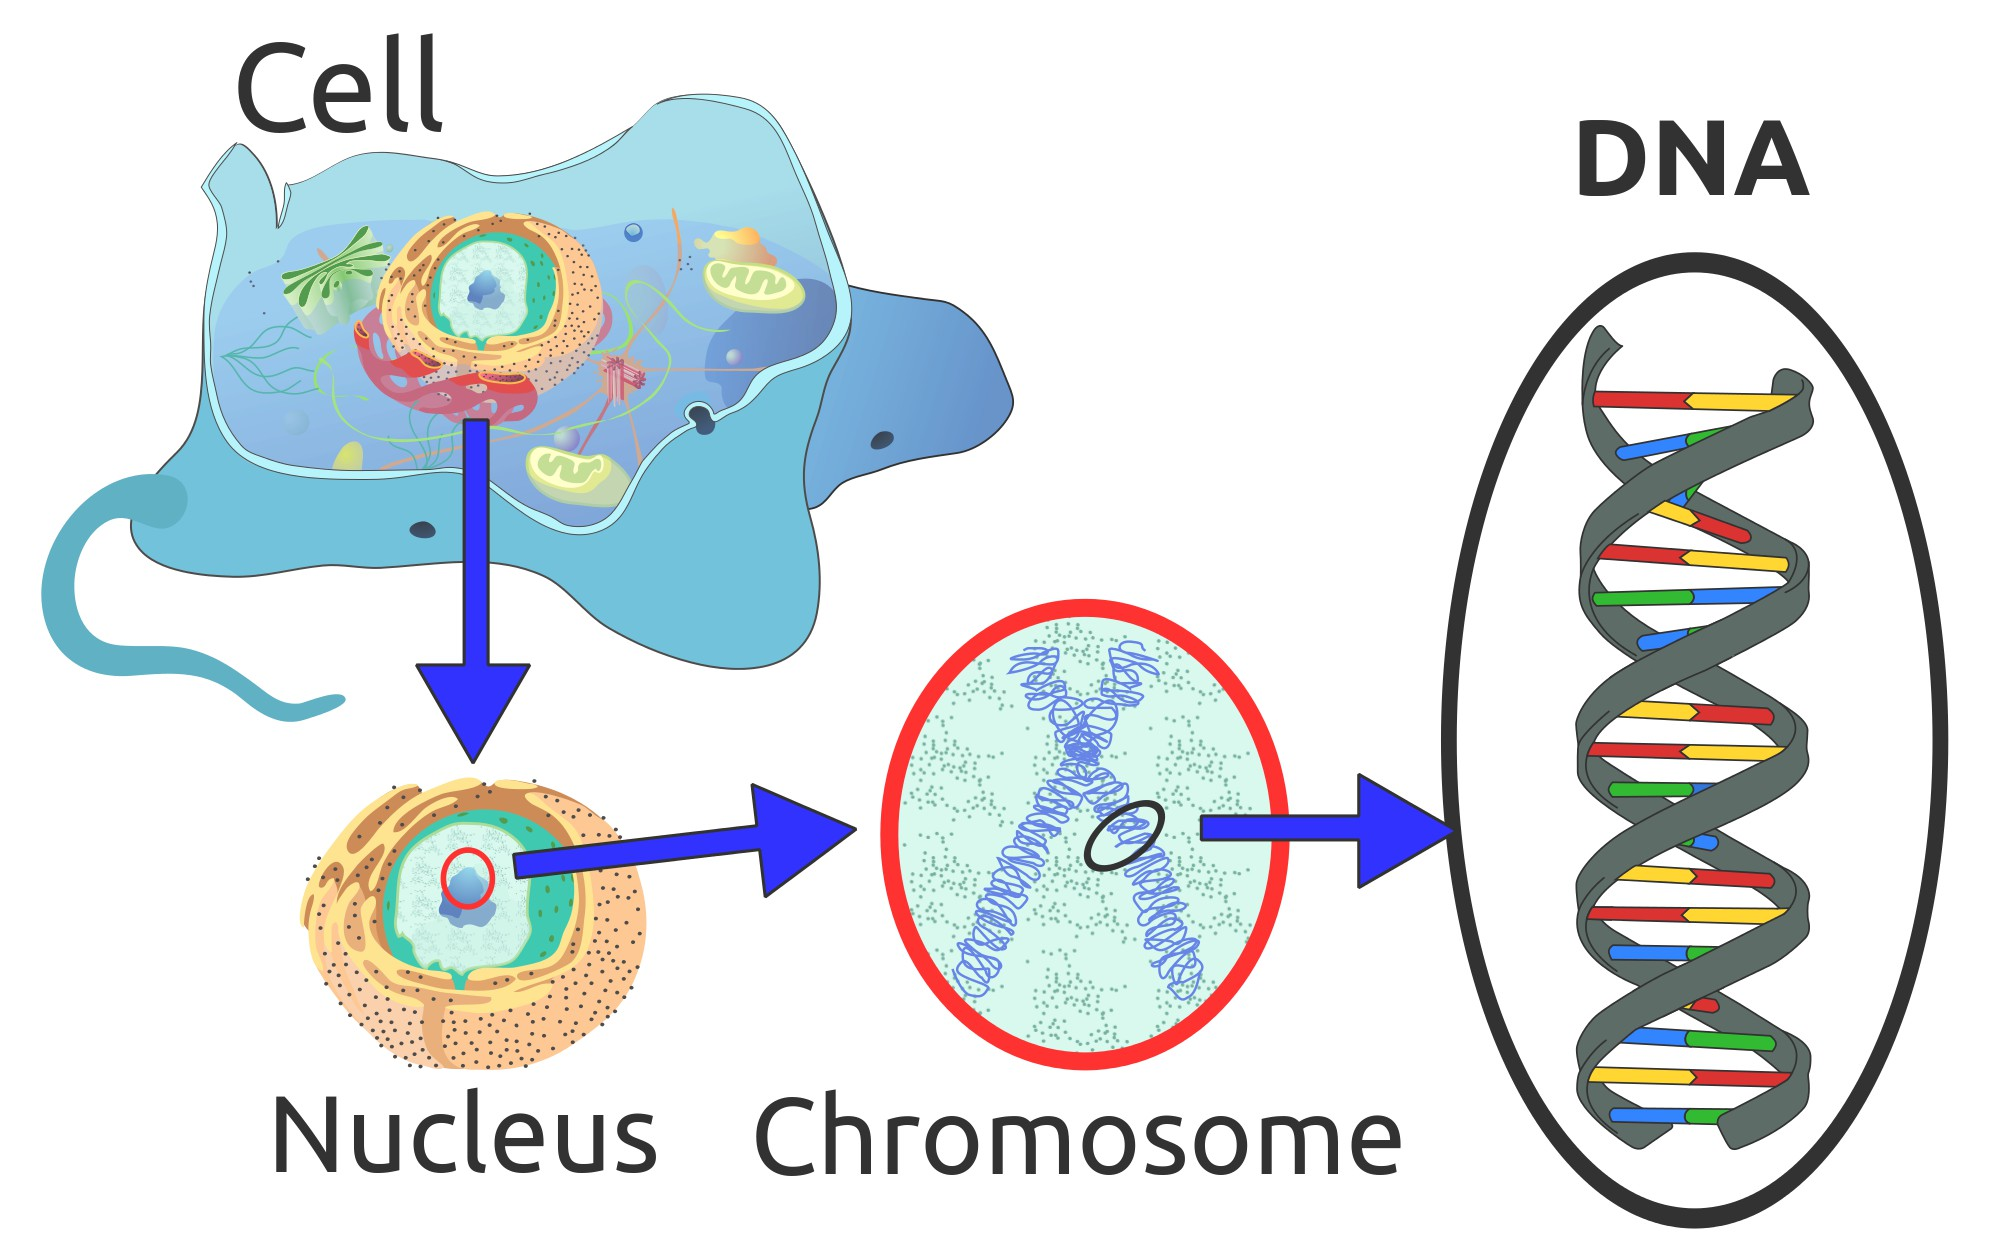
\includegraphics[width = 6cm]{Radiotherapy.jpg}
        \caption{caption.}
        \label{fig:1}
    \end{figure}

    \subsection{RBE (relative biological effectiveness)
 ფბე (ფარდობითი ბიოლოგიური ეფექტურობა) } 

	\begin{figure}[htp]
	    \centering
        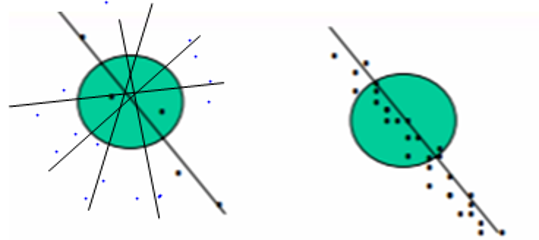
\includegraphics[width = 8cm]{Picture1.png}
        \caption{caption.}
        \label{fig:1}
    \end{figure}

\section{რადიაციული თერაპიის დაგეგმვა (Radiation Treatment Planing)}
\subsection{ფანტომები (Phantoms)}

\medskip

\printbibliography

\end{document}